%
\hsection{Example: Job Shop Scheduling Problem}%
\label{sec:jsspExample}%
%
Another typical optimization task arises in manufacturing, namely the assignment (\inQuotes{scheduling}) of tasks (\inQuotes{jobs}) to machines in order to optimize a given performance criterion (\inQuotes{objective}).
Scheduling~\cite{P2016STAAS,PS2009FYOSASOM} is one of the most active areas of operational research for more than  six decades.

In the \emph{Job Shop Scheduling Problem}~(JSSP)~\cite{CGLL1995STAIA,GLLRK1979OAAIDSASAS,LLRKS1993SASAAC,L1982RRITTOMS,T1993BFBSP,BDP1996TJSSPCANST}, we have a factory (\inQuotes{shop}) with several machines.
We receive a set of customer orders for products which we have to produce.
We know the exact sequence in which each product/order needs to pass through the machines and how long it will need at each machine.
Each production job has one production step (\inQuotes{operation}) for each machine on which it needs to be processed.
These operations must be performed in the right sequence.
Of course, no machine can process more than one operation at a time.
While we must obey these constraints, we can decide about the time at which each of the operations should begin.
Often, we are looking for the starting times that lead to the earliest completion of all jobs, i.e., the shortest makespan.

\begin{figure}%
\centering%
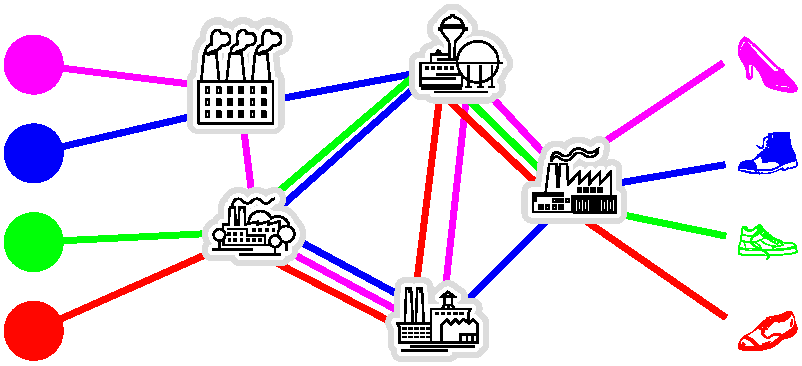
\includegraphics[width=0.75\linewidth]{\currentDir/jssp_sketch}%
\caption{Illustrative sketch of a JSSP scenario with four jobs where four different types of shoe should be produced, which require different workshops (\inQuotes{machines}) to perform different production steps.}%
\label{fig:jssp_sketch}%
\end{figure}%
%
Such a scenario is sketched in \autoref{fig:jssp_sketch}, where four orders for different types of shoe should be produced.
The resulting jobs pass through different workshops (or machines, if you want) in different order.
Some, like the green sneakers, only need to be processed by a subset of the workshops.

This general scenario encompasses many simpler problems.
For example, if we only produce one single product, then all jobs would pass through the same machines in the same order.
Customers may be able to order different quantities of the product, so the operations of the different jobs for the same machine may need different amounts of time.
This is the so-called Flow Shop Scheduling Problem (FSSP) --- and it has been defined back in 1954~\cite{J1954OTATSPSWSTI}!

Clearly, since the JSSP allows for an \emph{arbitrary} machine order per job, being able to solve the JSSP would also enable us to solve the FSSP, where the machine order is fixed.
We will introduce the JSSP in detail in TODO and use it as the main example in this book on which we will step-by-step exercise different optimization methods.%
\endhsection%
%
